\section{MIP model}


\subsection{Decision variables}

The MIP models also follow the same idea presented in \Cref{sec:intro}.
% In particular, taking inspiration from the AMPL book \cite{AMPLbook}, we model the Hamiltonian cycle by using a binary tensor that encodes the Hamiltonian cycle of each courier through all the possible delivery points, starting and ending at the depot. 
% This travel is an Hamiltonian cycle and we recall here the definition:
% \begin{definition}[Hamiltonian cycle]
% In the mathematical field of graph theory an Hamiltonian cycle (or Hamiltonian circuit) is a cycle that visits each vertex exactly once.
% \end{definition}
% In order to preserve the properties of the Hamiltonian cycle and to avoid the possible presence of sub-circuits we added some constraints, and in particular for the last case we followed the Miller–Tucker–Zemlin (MTZ) approach.\\
The models are based on the following three variables:
\begin{itemize}
    \item A binary tensor $X \in \{0,1\}^{(n+1) \times (n+1) \times m}$, where $X[i,j,k] = 1$ if and only if the courier $k$ depart from the $i$-th delivery point and arrive at the $j$-th one. This formulation is inspired from the AMPL book \cite{AMPLbook}.

    \item A binary matrix $A \in \{0,1\}^{n \times m}$, where $A[i,k] = 1$ if and only if the the package $i$ is delivered by the courier $k$. We observe that these variables are not strictly necessary for the model, but they allowed us to write some constraints in an easier way.

    \item An auxiliary matrix $u \in \{1,\dots,n+1\}^{(n+1) \times m}$ that keeps track of the order in which nodes are visited by each courier starting from $1$. It is necessary, following the MTZ formulation, for the sub-circuits elimination. The interpretation is that, fixing the courier $k$, $u[i,k] < u[j,k]$ implies that the node $i$ is visited before the node $j$ by the courier $k$.
\end{itemize}


\subsection{Objective function}
As objective function, defined from the assignment as the maximum distance travelled by any courier, we use the following: 
\begin{equation}
    \max_{k \in 1 \dots m}\sum_{i = 1}^{n+1} X[i,j,k] \cdot D[i,j]
\end{equation}
% As upper bound we chose the sum over all the indexes of the matrix $D$: $\sum_{i,j = 1}^{n+1} D[i,j]$. Instead as lower bound we chose the maximum distance travelled picking only one package: $\max_{i \in 1 \dots n} (D[n+1,i] + D[i,n+1])$. In fact, due to the triangular inequality, if another package is picked up by the courier the distance will grow. 

\subsection{Constraints}

We defined the following constraints:
\begin{itemize}
    \item Constraint to link the variables $A$ and $X$:
    \begin{equation}
        \sum_{j = 1}^{n+1} X[i,j,k] = A[i,k]  \qquad  \forall i \in 1 \dots n,\forall k \in 1 \dots m.
    \end{equation}
    \begin{equation}
        \sum_{i = 1}^{n+1} X[i,j,k] = A[j,k]  \qquad  \forall j \in 1 \dots n,\forall k \in 1 \dots m.
    \end{equation}

    \item Constraint to guarantee that each package has to be assigned:
    \begin{equation}
        \sum_{k = 1}^{m} A[i,k] = 1  \qquad \forall i \in 1 \dots n.
    \end{equation}

    \item Constraint for the capacity of each courier:
    \begin{equation}
        \sum_{i = 1}^{n} A[i,k] s[i] \leq l[k] \qquad \forall k \in 1 \dots m.
    \end{equation}

    \item Constraint to avoid that each courier departs and arrives at the same point:
    \begin{equation}
        X[i,i,k] = 0 \qquad \forall i \in 1 \dots n+1, \forall k \in 1 \dots m.
    \end{equation}

    % \item Two constraints to ensure that there is one arrival and one departure for each node, respectively. This concerns only the internal nodes because the depot is visited by each courier:
    % \begin{equation}
    %     \sum_{i \in 1 \dots n+1, k \in 1 \dots m} X[i,j,k] = 1 \qquad \forall j \in 1 \dots n.  
    % \end{equation}
    % \begin{equation}
    %     \sum_{j \in 1 \dots n+1, k \in 1 \dots m} X[i,j,k] = 1 \qquad \forall i \in 1 \dots n.  
    % \end{equation}

    \item Constraint for the preservation of the flow (if one courier arrives at one node, he departs from the same one):
    \begin{equation}
        \sum_{i = 1}^{n+1} X[i,j,k] = \sum_{i = 1}^{n+1} X[j,i,k] \qquad \forall j \in 1 \dots n, \forall k \in 1 \dots m.
    \end{equation}

    \item Constraints to ensure that each courier starts and ends its route at the depot:
    \begin{equation}
        \sum_{j = 1}^{n} X[n+1,j,k] = 1 \qquad \forall k \in 1 \dots m.
    \end{equation}
    \begin{equation}
        \sum_{j = 1}^{n} X[j,n+1,k] = 1 \qquad \forall k \in 1 \dots m.
    \end{equation}

    \item Constraints for MTZ subtour elimination:
    \begin{itemize}
        \item MTZ condition:
            \begin{equation}
            \makebox[\displaywidth]{$
                u[i,k] - u[j,k] + 1 \leq (n-1)(1 - X[i,j,k]) \qquad \forall i \in 1 \dots n, \forall j \in 1 \dots n+1, \forall k \in 1 \dots m.
            $}
            \end{equation}

        \item $u[i, k] = 1$ iff $i$ is the first item delivered by $k$:
            \begin{equation}
            \makebox[\displaywidth]{$
                u[i,k] \leq X[n+1,i,k] + (n+1)(1-X[n+1,i,k]) \qquad \forall i \in 1 \dots n, \forall k \in 1 \dots m.
            $}
            \end{equation}

        \item $u[j, k] \geq u[i, k] + 1$ iff $i$ is delivered before $j$:
            \begin{equation}
            \makebox[\displaywidth]{$
                u[j,k] \geq (u[i,k] + 1)X[i,j,k] \qquad \forall i \in 1 \dots n, \forall j \in 1 \dots n+1, \forall k \in 1 \dots m.
            $}
            \end{equation}
    \end{itemize}
    
    \subsubsection{Implied Model}
    For the implied model we added one more constraint with the same meaning of \Cref{eq:impl_constr}:
    \begin{equation}
        \sum_{i = 1}^{n} A[i,k] \geq 1 \qquad \forall k \in 1 \dots m.
    \end{equation}
    
    \subsubsection{Symmetry Model}
    For the symmetry model, we added the symmetry-breaking constraint related to the number of delivered packages as defined in \Cref{eq:cp_symm_amount}:
    \begin{equation}
        \sum_{i = 1}^{n} A[i,k] \leq \sum_{i = 1}^n A[i,j],
    \end{equation}
    where $k,j \in 1, \dots, m$ with $k < j$ and $l[k] = l[j]$.
\end{itemize}


\subsection{Validation}

\subsubsection{Experimental design}

For the MIP models, we choose to use the solver-independent language AMPL. The workflow is based on the construction of three different models: the initial one, the implied one and the symmetry one.

For reproducibility, we decided to only use open-source solvers such as HiGHS, SCIP, and GCG, provided by the AMPL framework.


\subsubsection{Experimental results}

Starting from some preliminary experiments, we immediately observed that GCG performs poorly on the first ten instances and therefore decided to discard it from the full experiments.

In \Cref{tab:mip_results}, we present the results of the MIP models. We can observe that the SCIP solver with the addition of the implied and symmetry breaking constraints improves in performance. On the other hand, this behavior is not the same for HiGHS.
Nevertheless, the HiGHS solver performances are in general significantly better than the SCIP ones.

\begin{table}[H]
    \centering
    \caption{Results of the SCIP and HiGHS solvers for the three models. Instances without a result have been omitted.}
    \label{tab:mip_results}
    \centerline{
        \begin{tabular}{ccccccc}
            \toprule
            Id & initial-scip & initial-highs & implied-scip & implied-highs & symmetry-scip & symmetry-highs \\ 
            \midrule
            1 & \textbf{14} &       \textbf{14} &   \textbf{14} &   \textbf{14} &   \textbf{14} &   \textbf{14} \\ 
            2 & \textbf{226} &      \textbf{226} &  \textbf{226} &  \textbf{226} &  \textbf{226} &  \textbf{226} \\

            3 & \textbf{12} &       \textbf{12} &   \textbf{12} &   \textbf{12} &   \textbf{12} &   \textbf{12} \\ 
            4 & \textbf{220} &      \textbf{220} &  \textbf{220} &  \textbf{220} &  \textbf{220} &  \textbf{220} \\

            5 & \textbf{206} &      \textbf{206} &  \textbf{206} &  \textbf{206} &  \textbf{206} &  \textbf{206} \\

            6 & \textbf{322} &      \textbf{322} &  \textbf{322} &  \textbf{322} &  \textbf{322} &  \textbf{322} \\

            7 & \textbf{167} &      \textbf{167} &  \textbf{167} &  \textbf{167} &  \textbf{167} &  \textbf{167} \\

            8 & \textbf{186} &      \textbf{186} &  \textbf{186} &  \textbf{186} &  \textbf{186} &  \textbf{186} \\

            9 & \textbf{436} &      \textbf{436} &  \textbf{436} &  \textbf{436} &  \textbf{436} &  \textbf{436} \\

            10 & \textbf{244} &     \textbf{244} &  \textbf{244} &  \textbf{244} &  \textbf{244} &  \textbf{244} \\

            13 & 642 &      726 &   616 &   694 &   526 &   692 \\
            16 & -- &       \textbf{286} &  -- &    557 &   -- &    320 \\
            \bottomrule
        \end{tabular}
    }
\end{table}


For the first ten instances, we plotted the graphs about the execution time (in seconds), the number of simplex iterations, and branching nodes explored for these two solvers.
\begin{figure}[H]
    \centering
    \begin{subfigure}{0.8\linewidth}
        \centering
        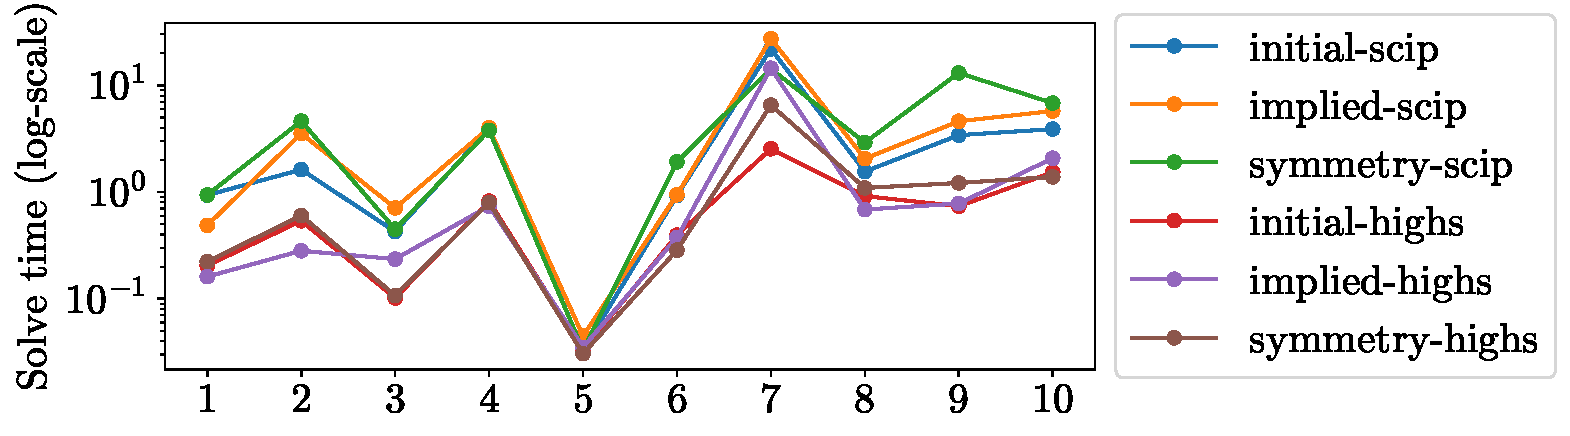
\includegraphics[width=\linewidth]{img/mip/time.pdf}
        % 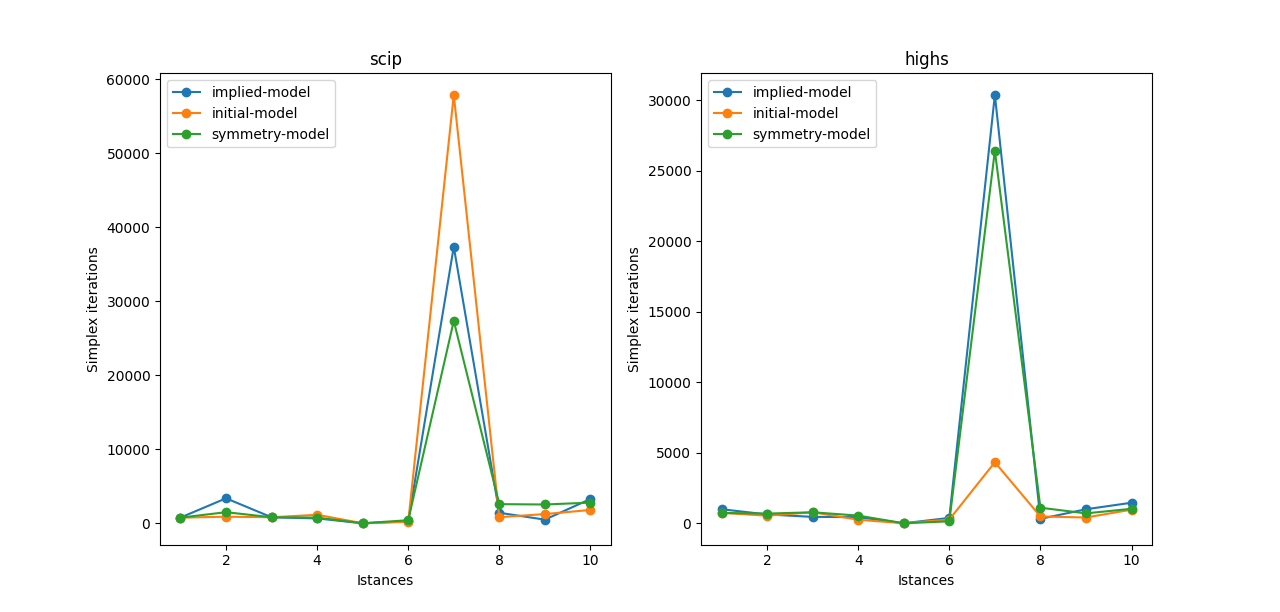
\includegraphics[width=\textwidth]{img/mip/simplex_iterations_2.png}
    \end{subfigure}
    \begin{subfigure}{0.8\linewidth}
        \centering
        % 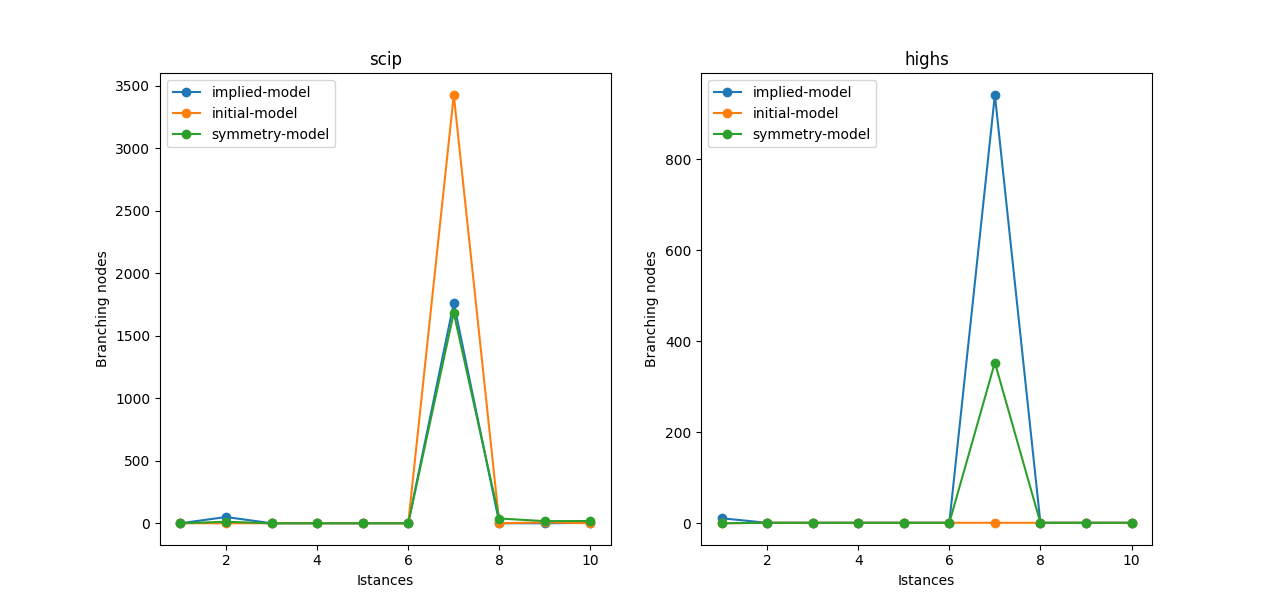
\includegraphics[width=\textwidth]{img/mip/Figure_2.png}
        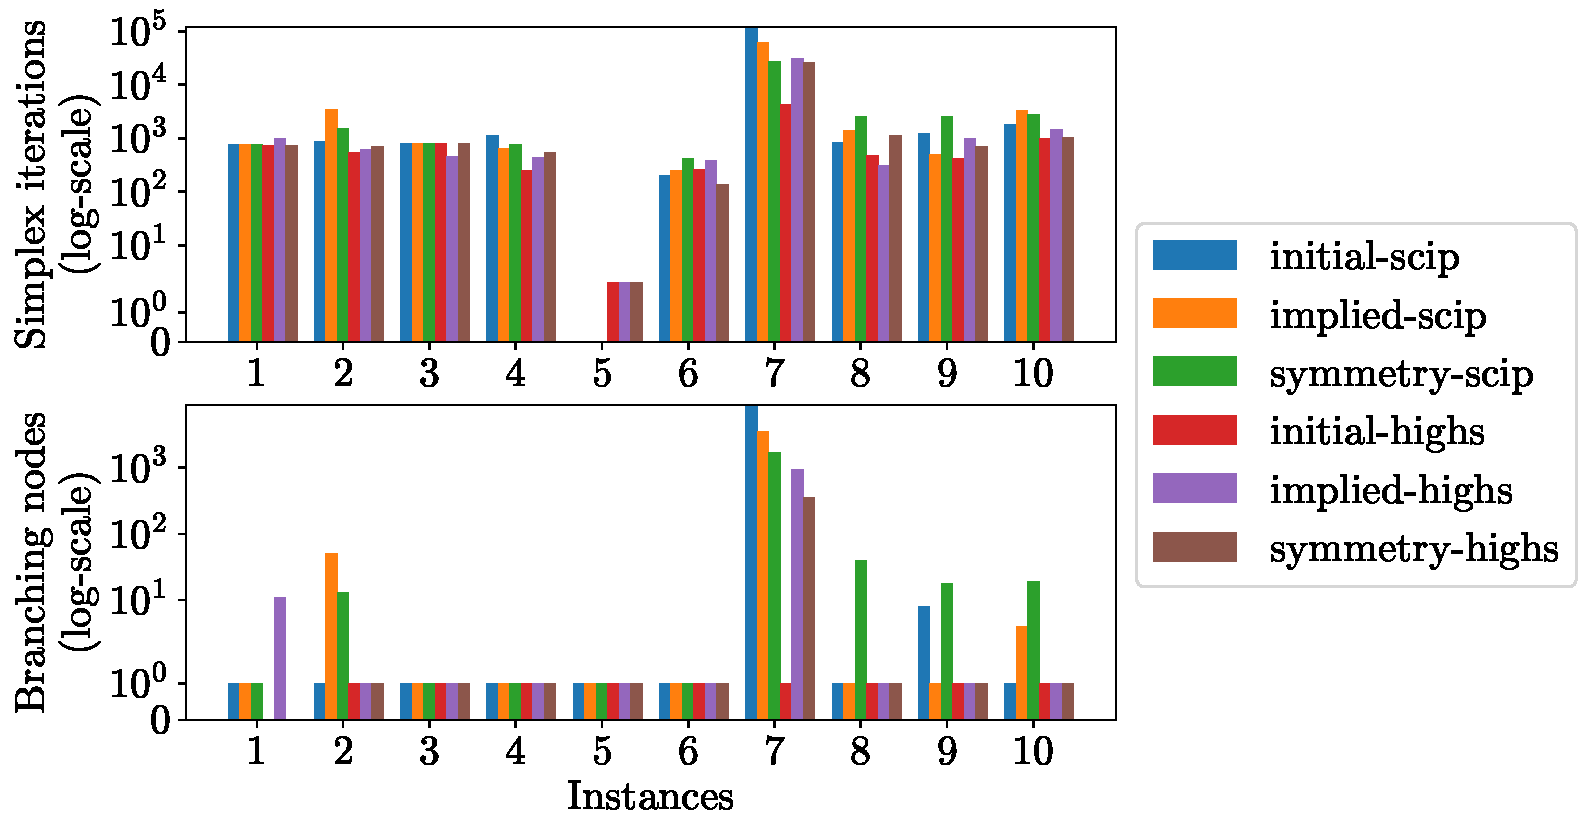
\includegraphics[width=\linewidth]{img/mip/simplex.pdf}
\end{subfigure}
    \caption{Compared statistics of the performances of the three models}
\end{figure}

% \begin{figure}[H]
%     \centering
%     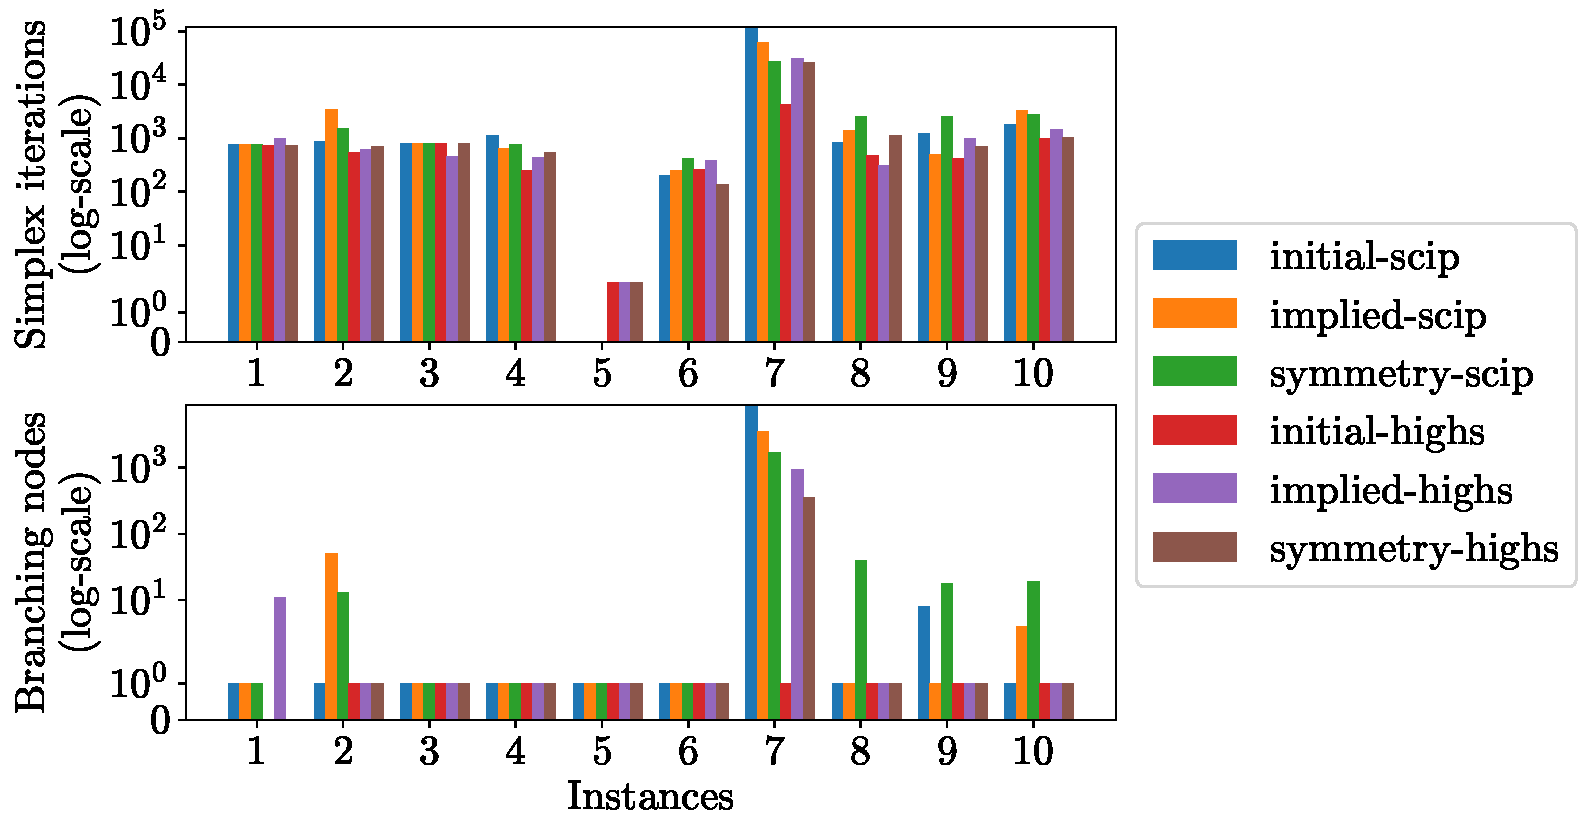
\includegraphics[width=\linewidth]{img/mip/simplex.pdf}
%     \caption{Compared statistics of the performances of the three models, divided by SCIP and HiGHS solvers.}
% \end{figure}


On a theoretical level, SCIP and HiGHS try to initially solve the relaxed-version of the problem (LP) using the revised simplex-method and finding a lower bound for the solution; then, if the solution found is not integer, they start to solve the MIP part using branch-and-cut (SCIP) or branch-and-bound (HiGHS). For the resolution of the sub-problems generated by these two methods, they proceed recursively by applying the same algorithm.
From the plots, we can observe that a lower number of simplex iterations and branching nodes corresponds to a faster resolution time. This is in line with our previous observation regarding HiGHS as a better performing solver.
